\documentclass[article,shortnames,nojss]{jss}\usepackage[]{graphicx}\usepackage[]{xcolor}
% maxwidth is the original width if it is less than linewidth
% otherwise use linewidth (to make sure the graphics do not exceed the margin)
\makeatletter
\def\maxwidth{ %
  \ifdim\Gin@nat@width>\linewidth
    \linewidth
  \else
    \Gin@nat@width
  \fi
}
\makeatother

\definecolor{fgcolor}{rgb}{0.345, 0.345, 0.345}
\newcommand{\hlnum}[1]{\textcolor[rgb]{0.686,0.059,0.569}{#1}}%
\newcommand{\hlstr}[1]{\textcolor[rgb]{0.192,0.494,0.8}{#1}}%
\newcommand{\hlcom}[1]{\textcolor[rgb]{0.678,0.584,0.686}{\textit{#1}}}%
\newcommand{\hlopt}[1]{\textcolor[rgb]{0,0,0}{#1}}%
\newcommand{\hlstd}[1]{\textcolor[rgb]{0.345,0.345,0.345}{#1}}%
\newcommand{\hlkwa}[1]{\textcolor[rgb]{0.161,0.373,0.58}{\textbf{#1}}}%
\newcommand{\hlkwb}[1]{\textcolor[rgb]{0.69,0.353,0.396}{#1}}%
\newcommand{\hlkwc}[1]{\textcolor[rgb]{0.333,0.667,0.333}{#1}}%
\newcommand{\hlkwd}[1]{\textcolor[rgb]{0.737,0.353,0.396}{\textbf{#1}}}%
\let\hlipl\hlkwb

\usepackage{framed}
\makeatletter
\newenvironment{kframe}{%
 \def\at@end@of@kframe{}%
 \ifinner\ifhmode%
  \def\at@end@of@kframe{\end{minipage}}%
  \begin{minipage}{\columnwidth}%
 \fi\fi%
 \def\FrameCommand##1{\hskip\@totalleftmargin \hskip-\fboxsep
 \colorbox{shadecolor}{##1}\hskip-\fboxsep
     % There is no \\@totalrightmargin, so:
     \hskip-\linewidth \hskip-\@totalleftmargin \hskip\columnwidth}%
 \MakeFramed {\advance\hsize-\width
   \@totalleftmargin\z@ \linewidth\hsize
   \@setminipage}}%
 {\par\unskip\endMakeFramed%
 \at@end@of@kframe}
\makeatother

\definecolor{shadecolor}{rgb}{.97, .97, .97}
\definecolor{messagecolor}{rgb}{0, 0, 0}
\definecolor{warningcolor}{rgb}{1, 0, 1}
\definecolor{errorcolor}{rgb}{1, 0, 0}
\newenvironment{knitrout}{}{} % an empty environment to be redefined in TeX

\usepackage{alltt}

%% -- LaTeX packages and custom commands ---------------------------------------

%% packages
\usepackage{thumbpdf,lmodern}
\usepackage{amsfonts,amsmath,amssymb,amsthm}
\usepackage{bbm,booktabs,setspace,longtable}
\usepackage[T1]{fontenc}
\usepackage{hyperref}
\usepackage{natbib}

%% custom commands
\newcommand{\class}[1]{`\code{#1}'}
\newcommand{\fct}[1]{\code{#1()}}

%\VignetteEngine{knitr::knitr}
%\VignetteIndexEntry{Standardised Energy Indices}
%\VignetteDepends{SEI}
%\VignetteKeywords{energy droughts, renewable energy production, residual load, standardised indices}
%\VignettePackage{SEI}
%\VignetteEncoding{UTF-8}

%\usepackage{Sweave}



%% -- Article metainformation (author, title, ...) -----------------------------

\author{Sam Allen\\University of Bern\\Oeschger Centre for \\Climate Change Research
\And Noelia Otero\\University of Bern\\Oeschger Centre for \\Climate Change Research}
\Plainauthor{Sam Allen, Noelia Otero}

\title{Calculating Standardised Indices Using \pkg{SEI}}
\Plaintitle{Calculating Standardised Indices Using SEI}
\Shorttitle{SEI}

\Abstract{
  Standardised indices are measurements of variables on a standardised scale. The standardised scale facilitates comparisons between different variables, and its probabilistic interpretation means the indices are effective for risk management and decision making. Standardised indices have become popular in weather and climate settings, for example within operational drought monitoring systems, and have also been applied in other contexts, such as to energy variables. To facilitate their implementation in practice, the \pkg{SEI} package in \proglang{R} allows the flexible calculation of standardised indices. This vignette discusses the theory underlying well-known standardised indices, outlines the general framework to construct them, and provides implementation details for the \pkg{SEI} package. Two case studies are presented whereby standardised indices are applied to climate and energy variables.
}

\Keywords{standardised indices, drought monitoring, energy droughts, \proglang{R}}
\Plainkeywords{standardised indices, drought monitoring, energy droughts, R}

\Address{
  Sam Allen\\
  University of Bern\\
  Institute of Mathematical Statistics and Actuarial Science\\
  Alpeneggstrasse 22\\
  3012 Bern, Switzerland\\
  E-Mail: \email{sam.allen@unibe.ch}\\
  \emph{and}\\
  Oeschger Centre for Climate Change Research\\

  Noelia Otero\\
  University of Bern\\
  Institute of Geography\\
  Hallerstrasse 12\\
  3012 Bern, Switzerland\\
  E-Mail: \email{noelia.otero@unibe.ch}\\
  \emph{and}\\
  Oeschger Centre for Climate Change Research\\
}

\newcommand{\R}{\mathbbm{R}}
\newcommand{\one}{\mathbbm{1}}
\IfFileExists{upquote.sty}{\usepackage{upquote}}{}
\begin{document}

\section{Introduction}\label{section:intro}

It is common to monitor the value of a variable over time: climate scientists monitor several weather and climate variables in the hope of identifying trends in the atmosphere; energy suppliers monitor energy demand and production, with particular focus recently on production from renewable sources; financial traders monitor financial indices to assess the behaviour of stock markets, and so on. Doing so allows practitioners to not only identify long term patterns in the variables of interest, but also to analyse abnormal situations with potentially adverse socio-economic consequences.

However, it can be difficult to compare time series of variables defined on different scales. For example, different spatial regions have different climates, meaning a rainfall event that is impactful at one location may not be at another. Similarly, energy demand will depend on the local climate, as well as on installed energy capacities. To account for this, it is convenient to transform variables onto the same, standardised scale. The resulting standardised variables are often referred to as \emph{standardised indices}.

Well-known examples of standardised indices include the Standardised Precipitation Index \citep[SPI;][]{McKeeEtAl1993} and Standardised Precipitation Evapotranspiration Index \citep[SPEI;][]{VicenteEtAl2010}, which are ubiquitously used to monitor hydrometeorological droughts \citep{BegueriaEtAl2014}. The framework used to construct the SPI and SPEI is simple and interpretable, framing the observed values in terms of their similarity to past values. As such, while other methods of standardisation exist, this framework has also been used to construct many other weather and climate indices.

This includes, for example, a Standardised Runoff Index \citep{ShuklaWood2008}, a Standardised Streamflow Index \citep{VicenteEtAl2012}, a Standardised Groundwater Index \citep{BloomfieldMarchant2013}, and a Standardised Temperature Index \citep{ZscheischlerEtAl2014}. Multivariate extensions of these standardised indices have also been proposed \citep{ErhardtCzado2018}. \cite{HaoEtAl2019}, for example, define a Standardised Compound Event Index, which is used by \cite{LiEtAl2021} to construct a Standardised Compound Drought and Heat Index. Outside of a weather and climate context, \cite{AllenOtero2023} introduced analogues of the SPI and SPEI that can be used to monitor energy supply and demand. This general framework for constructing standardised indices can be applied to any variable of interest, not just those previously considered in the literature.

There are several benefits to these standardised indices. The indices are easy to interpret, and are defined on a scale with a probabilistic interpretation, making them useful tools for risk management and decision making. Standardised indices therefore provide an appealing framework with which to define shortages, or droughts, in the variable of interest. Since the standardisation can be performed separately in different conditions, for example in different seasons and locations, these shortages can be defined in a relative sense, allowing their intensity in the different conditions to be compared. As summarised by \cite{ZargarEtAl2011}, standardised indices provide a ``pragmatic way to assimilate large amounts of data into a quantitative information that can be used in applications such as drought forecasting, declaring drought levels, contingency planning and impact assessment.''

As a result, several software packages have been developed to apply standardised indices in practice. The \pkg{SCI} package \citep{SCI} in the programming language \proglang{R} \citep{R} provides the functionality to calculate several standardised climate indices. The \pkg{SPEI} package \citep{SPEI-R}, also in \proglang{R}, contains more comprehensive functionality for the SPI and SPEI, and the \pkg{standard-precip} package \citep{standard-precip} has transferred this functionality to the programming language \proglang{Python} \citep{python}. The \pkg{spei} package \citep{spei-python} in \proglang{Python} additionally allows computation of the SPI and SPEI, as well as the Standardised Runoff and Groundwater Indices, while the \pkg{climate-indices} package in \proglang{Python} also provides functionality to compute the SPI, SPEI, and other drought indices. The developmental package \pkg{standaRdized} \citep{standaRdized} can also be used for this purpose, while the \pkg{SPIGA} package \citep{SPIGA} in \proglang{R} allows the SPI to be calculated using genetic algorithms.

However, existing software packages are limited in their flexibility, with functionality typically restricted to particular standardised indices (generally the SPI and SPEI), and particular assumptions about the reference data or parametric distributions used to calculate the indices (see next section for details). In this vignette, we introduce the \pkg{SEI} \proglang{R} package, which seeks to assimilate the advantages of these various packages to provide a flexible and comprehensive software package with which to calculate standardised indices. In particular, the package is not designed solely for climate indices, and is therefore applicable in much broader generality. The package can handle variables defined on any time scale and with any underlying distribution, permits user-specified reference data when calculating the indices, and additionally provides plot capabilities to visualise the resulting standardised indices.

The remainder of this vignette is organised as follows. Section \ref{section:theory} provides some theoretical background on standardised indices and describes the general formula to construct them. Section \ref{section:distribution} discusses diagnostic checks that confirm the standardisation was appropriate. Section \ref{section:functionality} demonstrates how the \pkg{SEI} package can be used to calculate standardised indices in practice. Two applications are then presented in Section \ref{section:application}, whereby the \pkg{SEI} package is used to calculate standardised energy indices based on time series of renewable energy production, as well as standardised wind speed indices. Section \ref{section:conclusion} concludes the vignette and discusses possible extensions to the package.


\section{How to construct standardised indices}\label{section:theory}

There is no unique way to define standardised indices. However, several widely-adopted indices are constructed using the same, simple procedure. Using this procedure, standardised indices are straightforward to calculate, can be defined on any timescale, and behave in a relative sense, meaning they can readily be compared for different variables, spatial regions, or points in time.

The general approach is to choose a univariate variable $X$ that measures the quantity of interest, and then to estimate $X$'s distribution: in the SPI, $X$ represents the precipitation accumulation aggregated over the time scale of interest, which is usually assumed to follow a gamma distribution; in the SPEI, $X$ represents the difference between precipitation and evapotranspiration, which is usually assumed to follow a log-logistic distribution; in the standardised temperature index, $X$ represents the temperature, which is usually assumed to follow a normal distribution. More complicated variables have also been considered. \cite{HaoEtAl2019}, for example, consider $X$ to be the probability of a simultaneously hot and dry event, as derived from a copula analysis.

The distribution of $X$ is typically estimated from an archive of realisations, $x_{1}, \dots, x_{n}$. These could represent precipitation accumulations in different months, for example, or energy demand on different days. It is common to make parametric assumptions about the distribution, as in the examples above, though non- and semi-parametric density estimation methods could also be employed. The choice of distribution is discussed in detail in the following section. In any case, the distributional assumptions must be verified when the index is calculated.

Let $F$ denote the distribution function of $X$, and let $\hat{F}$ denote an estimate of $F$ obtained from $x_{1}, \dots, x_{n}$. If $F$ is continuous, then the \emph{probability integral transform} (PIT) $F(X)$ will be standard uniformly distributed. Hence, this transformation provides a convenient approach with which to standardise an (new) observation $X^{*}$.

This \emph{PIT variable} $\hat{F}(X^{*})$ is bounded between 0 and 1, with values intrinsically linked to probabilities. This therefore itself provides a standardised index of sorts. This PIT variable can also be rescaled using $2\hat{F}(X^{*}) - 1$ to get an index that is centred at zero and bounded between -1 and 1, though it is more common to use the Gaussian quantile function $\Phi^{-1}$ to transform $\hat{F}(X^{*})$. In this case, if $X^{*}$ is identically distributed to $X$, and $\hat{F}$ is a good approximation of $F$, then the standardised index will follow a standard normal distribution.

That is, for any variable of interest, the probability integral transform can be used to define three different types of standardised indices:
\begin{itemize}
  \item \makebox[4cm]{\emph{Normal indices}: \hfill} $\Phi^{-1}(\hat{F}(X^{*}))$
  \item \makebox[4cm]{\emph{Probability indices}: \hfill} $\hat{F}(X^{*})$
  \item \makebox[4cm]{\emph{Bounded indices}: \hfill} $2\hat{F}(X^{*}) - 1$
\end{itemize}

All three types of indices can be calculated from observations of the variable $X$ and an estimate of its distribution $F$. In practice, it is most common to use normal indices, though one could argue that probability and bounded indices have a more direct probabilistic interpretation. For example, if we observe the 90$^{th}$ percentile of $X$, then (assuming $F$ is correctly estimated) the corresponding normal index will be 1.28, the 90$^{th}$ percentile of the standard normal distribution, whereas the probability index will be 0.9, and the bounded index will be 0.8. Similarly, for the 10$^{th}$ percentile of $X$, the normal index will be -1.28, the probability index will be 0.1, and the bounded index will be -0.8. For the median of $X$, the normal and bounded indices will be zero, whereas the probability index will be 0.5.

The general framework can therefore be summarised as follows.
\begin{enumerate}
  \item Estimate $F$ from the observations $x_{1}, \dots, x_{n}$.
  \item Check that the estimate $\hat{F}$ correctly fits the data.
  \item Apply $\hat{F}$ to an observation $X^{*}$ (or several observations).
  \item Transform $\hat{F}(X^{*})$ so that the index is on the desired scale.
\end{enumerate}

The probabilistic interpretation of these standardised indices has made them a useful tool when analysing shortages and excesses of the variable $X$. This was first proposed by \cite{McKeeEtAl1993} in the context of hydrometeorological droughts, and \cite{AllenOtero2023} demonstrate that the same framework can be employed to define droughts in energy systems. In this case, droughts are defined when the standardised index exceeds or falls below a relevant threshold. Different classes of droughts can be defined using different thresholds, with a more severe drought corresponding to a more extreme threshold.

Following \cite{McKeeEtAl1993}, it is most common to employ three categories, typically labelled ``Moderate'', ``Severe'', and ``Extreme'' droughts. These often correspond to the thresholds 1, 1.5, and 2 of the normal standardised indices, respectively, though the thresholds 1.28, 1.64, and 1.96 could also be used, which correspond to quantiles of the standard normal distribution. This assumes that a drought is defined as an exceedance of a threshold, though the negative of these values could analogously be used when interest is on values that fall below a threshold. Table \ref{tab:drought_def} gives corresponding threshold values for the other two types of indices.

\renewcommand*{\arraystretch}{1.5}
\begin{table}
    \centering
    \begin{tabular}{ l | c c c | c c c }
         & \multicolumn{3}{c |}{Exceed} & \multicolumn{3}{c}{Fall below} \\
        Index Type & Moderate & Severe & Extreme & Moderate & Severe & Extreme \\
        \hline
        Normal & 1.28 & 1.64 & 1.96 & -1.28 & -1.64 & -1.96 \\
        Probability & 0.9 & 0.95 & 0.975 & 0.1 & 0.05 & 0.025 \\
        Bounded & 0.8 & 0.9 & 0.95 & -0.8 & -0.9 & -0.95 \\
    \end{tabular}
    \caption{Possible thresholds used to define droughts when using each of the three types of standardised indices.}
    \label{tab:drought_def}
\end{table}

The \pkg{SEI} package allows the computation of all three types of indices, and additionally allows drought occurrences and characteristics to be computed from a time series of standardised indices.


\section{The choice of distribution}\label{section:distribution}

The construction of standardised indices relies on an estimate of the distribution function $F$. This has led to much debate about what distributional assumptions are most appropriate. Consider the SPI, for example.  \cite{McKeeEtAl1993} initially introduced the SPI using the gamma distribution to model $F$. However, \cite{Guttman1999} argued that the Pearson III distribution is more appropriate, due to the additional flexibility afforded by an extra parameter, while results in \cite{StaggeEtAl2015} suggest the Weibull distribution fits the monthly precipitation accumulations in their study better than alternative parametric choices. \cite{RussoEtAl2013} also consider using non-stationary distributions that include parameters that depend on time, while \cite{LiEtAl2015} incorporate additional covariates based on other climate variables. In reality, there is generally no true parametric distribution underlying the data, and the optimal assumptions will change depending on the data under consideration.

As an alternative, it has been argued \citep[e.g.][]{ErhardtCzado2018,HaoEtAl2019,AllenOtero2023} that the choice of a parametric distribution can be circumvented by using the empirical distribution function of the observations,
\begin{equation}\label{eq:ecdf}
\hat{F}_{n}(x) = \frac{1}{n} \sum_{i=1}^{n} \one \{ x_{i} \leq x \},
\end{equation}
where $\one\{ \cdot \}$ is equal to one if the statement inside the brackets is true, and zero otherwise. Since $\Phi^{-1}(0) = -\infty$ and $\Phi^{-1}(1) = \infty$, it is common to rescale $\hat{F}_{n}(x)$ so that it is never equal to zero or one, thereby ensuring that the (normal) standardised indices are real-valued; for example, using $(n \hat{F}_{n}(x) + 1)/(n + 2)$. The empirical distribution function returns a standardised index that can only take on $n + 1$ possible values. This is not an issue in practice if $n$ is large, but can become problematic with smaller sample sizes, particularly when interest is on extreme events.

\cite{AllenOtero2023} propose the use of semi-parametric density estimation methods, which provide a compromise between parsimonious parametric distributions and the empirical distribution function. For example, kernel density estimators estimate the density function $f$ corresponding to $F$ using
\[
\hat{f}(x) = \frac{1}{nh} \sum_{i=1}^{n} K \left( \frac{x - x_{i}}{h} \right),
\]
where $K$ is a kernel function, and $h > 0$ is a smoothing parameter called the bandwidth. The \pkg{SEI} package provides functionality to perform kernel density estimation using a Gaussian kernel. Non- and semi-parametric density estimation methods are considerably more flexible than parametric methods, though they require more data to accurately model $F$. Further details about density estimation methods can be found, for example, in \cite{Silverman2018}.

\renewcommand*{\arraystretch}{1.5}
\begin{table}
    \centering
    \begin{tabular}{ l | l | c }
        Distribution & Argument code & Support \\
        \hline
        Empirical & \code{"empirical"} & range$(x_{1}, \dots, x_{n})$ \\
        Kernel density estimation & \code{"kde"} & $\R$ \\
        Normal & \code{"norm"} & $\R$ \\
        Log-normal & \code{"lnorm"} & $[0, \infty)$ \\
        Logistic & \code{"logis"} & $\R$ \\
        Log-logistic & \code{"llogis"} & $[0, \infty)$ \\
        Exponential & \code{"exp"} & $[0, \infty)$ \\
        Gamma & \code{"gamma"} & $[0, \infty)$ \\
        Weibull & \code{"weibull"} & $[0, \infty)$ \\
    \end{tabular}
    \caption{Distributions available in \pkg{SEI}, and their supports.}
    \label{tab:dists}
\end{table}

Table \ref{tab:dists} lists the distributions available in the \pkg{SEI} package for estimating $F$. The choice of distribution should align with the variable of interest. For example, if interest is on precipitation, then we should not choose a distribution that assigns positive probability density to negative values, such as the normal distribution. Conversely, if interest is on temperature (in Celsius), then we should not choose a distribution that has support $[0, \infty)$, such as the exponential distribution. Table \ref{tab:dists} additionally contains the support of the available distributions; the support of the empirical distribution is determined by the archive of observations $x_{1}, \dots, x_{n}$. Wherever relevant, $\hat{F}$ is estimated using maximum likelihood estimation.

Regardless of the method used to estimate $F$, it is necessary to check that the estimated distribution fits the data. Several goodness-of-fit tests exist for this purpose. The \pkg{SEI} package implements the Kolmogorov-Smirnov test \citep{Massey1951}, which is based on the test statistic
\begin{equation}\label{eq:kolsmi}
  \sup_{x \in \R} | \hat{F}_{n}(x) - \hat{F}(x) |,
\end{equation}
that is, the maximum difference between the estimated distribution function $\hat{F}$ and the empirical distribution function $\hat{F}_{n}$. If this statistic is close to zero, then it suggests that the hypothesised distribution fits the data well. Clearly, if the empirical distribution is used to estimate $F$, then this test statistic is zero.

The fit of the distribution could also be visualised graphically by plotting the PIT values $\hat{F}(x_{1}), \dots, \hat{F}(x_{n})$ or the corresponding standardised indices. If the model fits the data well, then these PIT values should resemble a sample from a standard uniform distribution; a histogram of these values should therefore be flat, up to sampling variation. Similarly, the normal standardised indices should resemble a sample from a standard normal distribution. An example of how this can be checked using the \pkg{SEI} package is presented in Section \ref{section:application}.


\section{Package functionality}\label{section:functionality}

\subsection{Standardised indices}

The \pkg{SEI} package is designed to facilitate the computation of standardised indices. The principal function in the package is \code{std_index()}, which takes a time series or vector \code{x_new} as an input, and returns a time series or vector of corresponding standardised index values.

\begin{Code}
std_index(
  x_new,
  x_ref = x_new,
  timescale = NULL,
  dist = "empirical",
  return_fit = FALSE,
  moving_window = NULL,
  window_scale = NULL,
  agg_period = NULL,
  agg_scale = NULL,
  agg_fun = "sum",
  rescale = NULL,
  rescale_fun = "sum",
  index_type = "normal",
  ignore_na = FALSE
)
\end{Code}

The input \code{x_new} must be either a vector or an \pkg{xts} time series object. The argument \code{x_ref} is similarly a vector or time series, containing the archive $x_{1}, \dots, x_{n}$ of past observations that are used to estimate the distribution $F$. This distribution is then applied to each value in \code{x_new}, which therefore correspond to values of $X^{*}$ in the previous section. The default is that \code{x_ref = x_new}, in which case the standardised indices are calculated \emph{in-sample}.

As a very simple example, consider a vector of observations drawn from a gamma distribution. These can be converted to (normal) standardised indices as follows.

\begin{knitrout}
\definecolor{shadecolor}{rgb}{0.969, 0.969, 0.969}\color{fgcolor}\begin{kframe}
\begin{alltt}
\hlstd{x} \hlkwb{<-} \hlkwd{rgamma}\hlstd{(}\hlnum{1000}\hlstd{,} \hlkwc{shape} \hlstd{=} \hlnum{2}\hlstd{,} \hlkwc{scale} \hlstd{=} \hlnum{1}\hlstd{)}
\hlstd{x_std} \hlkwb{<-} \hlkwd{std_index}\hlstd{(x)}
\end{alltt}
\end{kframe}
\end{knitrout}

Histograms of the raw and standardised values are displayed in Figure \ref{fig:hist_ex}. While the raw values are heavily skewed, the standardised values closely resemble a standard normal distribution.

\begin{figure}
\begin{knitrout}
\definecolor{shadecolor}{rgb}{0.969, 0.969, 0.969}\color{fgcolor}\begin{kframe}
\begin{alltt}
\hlstd{plot_raw} \hlkwb{<-} \hlkwd{plot_sei}\hlstd{(x,} \hlkwc{type} \hlstd{=} \hlstr{"hist"}\hlstd{,} \hlkwc{title} \hlstd{=} \hlstr{"Raw"}\hlstd{)}
\hlstd{plot_std} \hlkwb{<-} \hlkwd{plot_sei}\hlstd{(x_std,} \hlkwc{type} \hlstd{=} \hlstr{"hist"}\hlstd{,} \hlkwc{title} \hlstd{=} \hlstr{"Standardised"}\hlstd{)}
\hlkwd{grid.arrange}\hlstd{(plot_raw, plot_std,} \hlkwc{nrow} \hlstd{=} \hlnum{1}\hlstd{)}
\end{alltt}
\end{kframe}

{\centering 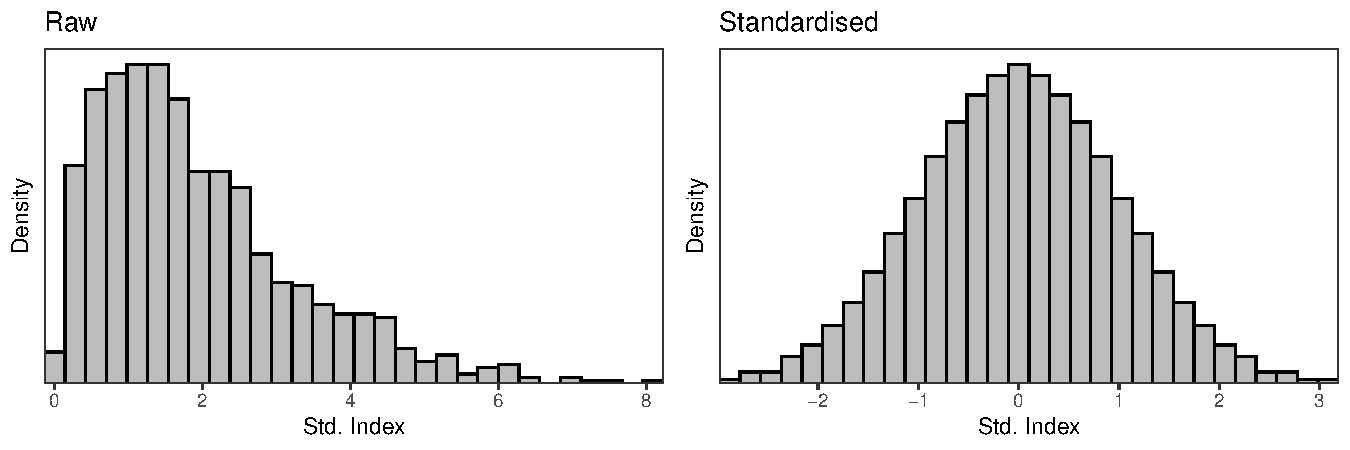
\includegraphics[width=\linewidth]{figure/std_index_ex_plot-1} 

}


\end{knitrout}
\caption{Histogram of values sampled from a gamma distribution, and corresponding standardised values.}
\label{fig:hist_ex}
\end{figure}

The \code{dist} argument in \code{std_index()} specifies how the distribution $F$ will be estimated from \code{x_ref}. The default is to use the empirical distribution of \code{x_ref} (Equation \ref{eq:ecdf}). To accurately estimate $F$, the empirical distribution requires a sufficiently large archive, and a warning is therefore returned if the length of \code{x_ref} is smaller than 100. An error message is returned if the distribution support does not align with the data; for example, if a distribution with support $[0, \infty)$ is chosen while the data contains negative values.

Information about the distribution fit, including estimated parameters and goodness-of-fit statistics, can be returned by setting \code{return_fit = TRUE}; the default is \code{return_fit = FALSE}. If \code{return_fit = TRUE}, the output of \code{std_index()} is a list containing the time series of standardised indices (\code{si}), the estimated distribution parameters (\code{params}), and a named vector containing properties of the model fit (\code{fit_props}); this includes the number of observations used to estimate the distribution, the number and percentage of \code{NA} values in the data, the Akaike Information Criterion (AIC) value, and the p-value of the Kolmogorov-Smirnov test that the distribution correctly fits the data (Equation \ref{eq:kolsmi}).

The distribution fitting is performed using \code{fit_dist()}, which is essentially a wrapper for \code{fitdist()} in the \pkg{fitdistrplus} package, along with extensions that are relevant for the construction of standardised indices. The \code{fit_dist()} function is also exported by \pkg{SEI}, and further details can be found on the associated help page.

The argument \code{index_type} in \code{std_index()} specifies which type of standardised index should be used. This must be one of \code{"normal"} (the default), \code{"probability"}, or \code{"bounded"}, corresponding to the three definitions in the previous section.

The remaining arguments are only applicable when \code{x_new} and \code{x_ref} are time series, rather than vectors, since they all involve manipulations based on the date of the data. For example, the argument \code{moving_window} can be used to calculate standardised indices using a moving window. In this case, \code{x_ref} is updated for each observation in \code{x_new} so that it contains the previous \code{moving_window} (an integer) observations in the time series; the indices are therefore determined relative to recently observed values. The argument \code{window_scale} specifies the timescale that \code{moving_window} refers to. For example, setting \code{moving_window = 10} and \code{window_scale = "days"} would calculate standardised indices using a moving window of length 10 days.

If \code{moving_window} is specified but \code{window_scale = NULL}, then it is assumed that the units of \code{moving_window} correspond to the timescale of \code{x_new}. If the time difference between consecutive observations is consistent throughout the time series, then this can be determined automatically within \code{std_index()}. Alternatively, and more robustly, it can be specified by the user using the \code{timescale} argument. This (and \code{window_scale}) must be one of \code{"hours"}, \code{"days"}, \code{"weeks"}, \code{"months"}, \code{"quarters"}, or \code{"years"}.

If the original time series contains, say, hourly data, but the time series of standardised indices is desired on a different timescale, then the \code{rescale} argument can be used to rescale the data. This must also be one of the timescales listed above. By default, \code{std_index()} assumes the sum of the values should be returned when rescaling. For example, if interest is on precipitation accumulations, then converting hourly data to daily data will return the daily aggregations. However, alternative rescaling could also be performed using the \code{rescale_fun} argument, which is a function specifying what operation to perform over the aggregated data. If \code{rescale_fun = "mean"} or \code{rescale_fun = "max"}, for example, then the daily (or weekly, monthly, etc) mean or maximum would be provided, respectively, in place of the hourly data.

Similarly, the \code{agg_period} argument can be used to aggregate data across multiple time steps. Like \code{moving_window} and \code{window_scale}, \code{agg_period} is an integer representing the number of previous time steps over which the data should be aggregated, while \code{agg_scale} specifies the timescale of the aggregation period, which is by default assumed to be the timescale of the data. The argument \code{agg_fun} represents the function used to aggregate the data over the aggregation period.

This differs from \code{rescale} in the following way. If we want to convert a time series of daily observations to a time series of weekly indices, then we can use \code{rescale = "weeks"} (and \code{timescale = "days"}). On the other hand, if we set \code{agg_period = 1} and \code{agg_scale = "weeks"}, then we get a daily time series of weekly aggregated data.

To perform the rescaling, \code{std_index()} calls one of the \pkg{xts} functions \code{apply.daily}, \code{apply.weekly}, \code{apply.monthly}, \code{apply.quarterly}, and \code{apply.yearly}, alongside the argument \code{rescale_fun}. To perform the aggregation, \code{std_index()} uses the function \code{aggregate_xts()}, which is additionally exported by \pkg{SEI}.

\begin{Code}
aggregate_xts(
  x,
  len,
  scale = c("days", "hours", "weeks", "quarters", "years"),
  fun = "sum",
  timescale = c("days", "hours", "weeks", "quarters", "years"),
  na_thres = 10
)
\end{Code}

The interpretation of the arguments is equivalent to in the discussion above: \code{x} represents the \pkg{xts} time series to be aggregated, \code{len} and \code{scale} are the length and time scale of the aggregation period, \code{fun} is the function used in the aggregation, and \code{timescale} is the time scale of \code{x}. The final argument \code{na_thres} represents the maximum proportion of values that can be missing (i.e. \code{NA}) in the aggregation period, before the aggregation itself returns \code{NA}. For example, if 23 hours of precipitation accumulations are missing on one day so that only one hourly accumulation is available, this sole observation is not representative of the daily accumulation. By default, \code{NA} is returned if more than 10\% of the values in the aggregation period are missing.


\subsection{Plotting indices}

To visualise the indices, \pkg{SEI} includes the \code{plot_sei()} function.

\begin{Code}
plot_sei(
  x,
  type = c("ts", "hist"),
  title = NULL,
  lab = "Std. Index",
  xlims = NULL,
  ylims = NULL,
  n_bins = 30
)
\end{Code}

The argument \code{x} is either a vector or an \pkg{xts} time series object that contains the index values to be displayed. This function can either be used to plot a time series of the values (\code{type = "ts"}), or a histogram (\code{type = "hist"}). A time series can only be plotted if the input \code{x} is a time series and not a vector. If \code{type = "hist"}, the function is essentially a wrapper for \code{geom_histogram()} in \pkg{ggplot2}. Here, \code{n_bins} can be used to specify the number of bins in the histogram.

Additional aspects of the plot can be specified using \code{title}, \code{lab}, \code{xlims} and \code{ylims}. For the time series plot, \code{lab} refers to the label of the y-axis, whereas it corresponds to the x-axis label of the histogram.


\subsection{Drought definitions}

Having obtained a time series of standardised indices, one might wish to perform an analysis of shortages, or droughts, in the variable of interest. As discussed, this can be achieved using standardised indices with the definitions of droughts in Table \ref{tab:drought_def}. To facilitate such analyses, the \code{get_drought()} function takes a time series or vector \code{x} as input, and outputs a dataframe containing information regarding drought occurrences and characteristsics.

\begin{Code}
get_drought(x, thresholds = c(1.28, 1.64, 1.96), exceed = TRUE, lag = FALSE)
\end{Code}


The argument \code{thresholds} is a vector containing the thresholds used to define the droughts; by default, these correspond to the 90$^{th}$, 95$^{th}$, and 97.5$^{th}$ percentiles of a standard normal distribution. It is also assumed by default that a drought is defined when the standardised indices exceed these thresholds. This can be specified using the \code{exceed} argument. If a drought should instead correspond to an instance where the indices fall below the given thresholds, \code{exceed} should be \code{FALSE}.

When defining meteorological droughts, it is often common to introduce a lag such that the drought does not end when the standardised index no longer exceeds the drought threshold, but rather when the index changes sign \citep[e.g.][]{McKeeEtAl1993}. This accounts for cases where there are small fluctuations in the index around the drought threshold, classing this as one persistent drought rather than several shorter droughts. This can also be implemented here by setting the \code{lag} argument to \code{TRUE}.

The output is a dataframe containing the original vector or time series, as well as four additional columns: the intensity (\code{ins}), which corresponds to the category of drought, a higher value referring to a more severe drought category; the occurrence (\code{occ}), which corresponds to the intensity being higher than zero; the duration (\code{dur}), which provides the number of consecutive time steps that are in a drought state; and the drought magnitude (\code{mag}), which is the sum of all indices within the drought event \citep[see][for details]{McKeeEtAl1993}. If only one threshold is used to define a drought, rather than the three used in Table \ref{tab:drought_def}, then the intensity is equivalent to the occurrence, and is therefore not returned.


\section{Applications}\label{section:application}

\subsection{Renewable energy production}

Consider an application of standardised indices to renewable energy production in Europe. Hourly time series of wind and solar power generation are publicly available for 27 European countries at \url{https://researchdata.reading.ac.uk/275/} \citep[see][for details]{BloomfieldEtAl2020}. A subset of this data corresponding to production in 2019 can be accessed from \pkg{SEI} using

\begin{knitrout}
\definecolor{shadecolor}{rgb}{0.969, 0.969, 0.969}\color{fgcolor}\begin{kframe}
\begin{alltt}
\hlkwd{data}\hlstd{(}\hlstr{"data_supply"}\hlstd{,} \hlkwc{package} \hlstd{=} \hlstr{"SEI"}\hlstd{)}
\hlkwd{head}\hlstd{(data_supply)}
\end{alltt}
\begin{verbatim}
##                  date country        PWS
## 1 2019-01-01 00:00:00 Austria 0.07823861
## 2 2019-01-01 01:00:00 Austria 0.05330285
## 3 2019-01-01 02:00:00 Austria 0.06773745
## 4 2019-01-01 03:00:00 Austria 0.09971320
## 5 2019-01-01 04:00:00 Austria 0.18676895
## 6 2019-01-01 05:00:00 Austria 0.29001299
\end{verbatim}
\end{kframe}
\end{knitrout}

The dataframe \code{data_supply} contains a \code{POSIXct} time series of dates, along with the corresponding country and wind and solar power production (\code{PWS}). The units of the production are Gigawatt hours (GWh).

For concision, we restrict attention here to renewable energy production in Germany.

\begin{knitrout}
\definecolor{shadecolor}{rgb}{0.969, 0.969, 0.969}\color{fgcolor}\begin{kframe}
\begin{alltt}
\hlstd{de_supply_h} \hlkwb{<-} \hlkwd{subset}\hlstd{(data_supply, country} \hlopt{==} \hlstr{"Germany"}\hlstd{)}
\hlstd{de_supply_h} \hlkwb{<-} \hlstd{xts}\hlopt{::}\hlkwd{xts}\hlstd{(de_supply_h}\hlopt{$}\hlstd{PWS, de_supply_h}\hlopt{$}\hlstd{date)} \hlcom{# convert to xts}
\end{alltt}
\end{kframe}
\end{knitrout}

This can be rescaled from hourly to daily or weekly time series using \pkg{xts} functionality.

\begin{knitrout}
\definecolor{shadecolor}{rgb}{0.969, 0.969, 0.969}\color{fgcolor}\begin{kframe}
\begin{alltt}
\hlstd{de_supply_d} \hlkwb{<-} \hlstd{xts}\hlopt{::}\hlkwd{apply.daily}\hlstd{(de_supply_h,} \hlstr{"sum"}\hlstd{)}    \hlcom{# daily data}
\hlstd{de_supply_w} \hlkwb{<-} \hlstd{xts}\hlopt{::}\hlkwd{apply.weekly}\hlstd{(de_supply_h,} \hlstr{"sum"}\hlstd{)}   \hlcom{# weekly data}
\end{alltt}
\end{kframe}
\end{knitrout}

These time series of renewable energy production in Germany can be visualised using the \code{plot_sei()} function. Figure \ref{fig:ts_raw} demonstrates that all three time series display the same patterns, though the weekly time series removes the hourly and daily fluctuations.

\begin{figure}
\begin{knitrout}
\definecolor{shadecolor}{rgb}{0.969, 0.969, 0.969}\color{fgcolor}\begin{kframe}
\begin{alltt}
\hlstd{lab} \hlkwb{<-} \hlstr{"Renewable Energy Production (GWh)"}
\hlstd{plot_h} \hlkwb{<-} \hlkwd{plot_sei}\hlstd{(de_supply_h,} \hlkwc{lab} \hlstd{= lab,} \hlkwc{title} \hlstd{=} \hlstr{"Hourly"}\hlstd{)}
\hlstd{plot_d} \hlkwb{<-} \hlkwd{plot_sei}\hlstd{(de_supply_d,} \hlkwc{lab} \hlstd{= lab,} \hlkwc{title} \hlstd{=} \hlstr{"Daily"}\hlstd{)}
\hlstd{plot_w} \hlkwb{<-} \hlkwd{plot_sei}\hlstd{(de_supply_w,} \hlkwc{lab} \hlstd{= lab,} \hlkwc{title} \hlstd{=} \hlstr{"Weekly"}\hlstd{)}
\hlkwd{grid.arrange}\hlstd{(plot_h, plot_d, plot_w,} \hlkwc{nrow} \hlstd{=} \hlnum{1}\hlstd{)}
\end{alltt}
\end{kframe}

{\centering 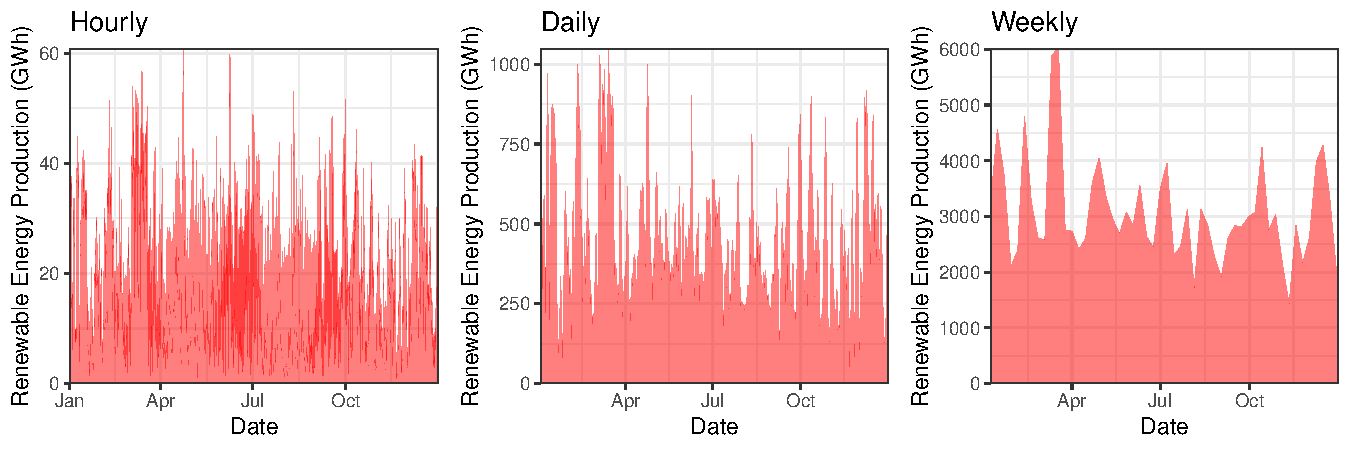
\includegraphics[width=\linewidth]{figure/plot_raw_ts-1} 

}


\end{knitrout}
\caption{Time series of 2019 renewable energy production in Germany at hourly, daily, and weekly time scales.}
\label{fig:ts_raw}
\end{figure}



The raw renewable energy production values can be transformed to a standardised index using \code{std_index()}. Following, \cite{AllenOtero2023}, we refer to this as the standardised renewable energy production index (SREPI). Time series of hourly, daily, and weekly standardised indices are presented in Figure \ref{fig:ts_si}.

\begin{knitrout}
\definecolor{shadecolor}{rgb}{0.969, 0.969, 0.969}\color{fgcolor}\begin{kframe}
\begin{alltt}
\hlstd{srepi_h} \hlkwb{<-} \hlkwd{std_index}\hlstd{(de_supply_h)}
\end{alltt}


{\ttfamily\noindent\bfseries\color{errorcolor}{\#\# Error in shapiro.test(qnorm(pit)): sample size must be between 3 and 5000}}\begin{alltt}
\hlstd{srepi_d} \hlkwb{<-} \hlkwd{std_index}\hlstd{(de_supply_d)}
\hlstd{srepi_w} \hlkwb{<-} \hlkwd{std_index}\hlstd{(de_supply_w,} \hlkwc{dist} \hlstd{=} \hlstr{"kde"}\hlstd{)}
\end{alltt}
\end{kframe}
\end{knitrout}

In this case, the reference data \code{x_ref} is assumed to be the input time series itself, meaning the indices are calculated relative to this input data. By default, \code{std_index()} returns normal indices (rather than probability or bounded indices), and estimates the distribution of the renewable energy production using the empirical distribution. This returns a warning for the weekly data, since there are fewer than 100 weekly production values in the time series, whereas the empirical distribution function is only recommended if at least 100 reference values are available. Instead, for weekly data, we estimate the distribution of production values using kernel density estimation (\code{dist = "kde"}). Alternative distributions can be implemented by changing the \code{dist} argument in \code{std_index()}.

While these indices are created by standardising the respective hourly, daily, and weekly time series of raw production values, they could all be obtained from the original hourly time series by specifying the \code{rescale} argument in \code{std_index()}.

\begin{knitrout}
\definecolor{shadecolor}{rgb}{0.969, 0.969, 0.969}\color{fgcolor}\begin{kframe}
\begin{alltt}
\hlstd{z} \hlkwb{<-} \hlkwd{std_index}\hlstd{(de_supply_h,} \hlkwc{rescale} \hlstd{=} \hlstr{"days"}\hlstd{)}
\hlkwd{all.equal}\hlstd{(srepi_d, z)}
\end{alltt}
\begin{verbatim}
## [1] TRUE
\end{verbatim}
\end{kframe}
\end{knitrout}

\begin{figure}
\begin{knitrout}
\definecolor{shadecolor}{rgb}{0.969, 0.969, 0.969}\color{fgcolor}\begin{kframe}
\begin{alltt}
\hlstd{lab} \hlkwb{<-} \hlstr{"SREPI"}
\hlstd{ylims} \hlkwb{<-} \hlkwd{c}\hlstd{(}\hlopt{-}\hlnum{3}\hlstd{,} \hlnum{3}\hlstd{)}
\hlstd{plot_h} \hlkwb{<-} \hlkwd{plot_sei}\hlstd{(srepi_h,} \hlkwc{lab} \hlstd{= lab,} \hlkwc{ylims} \hlstd{= ylims,} \hlkwc{title} \hlstd{=} \hlstr{"Hourly"}\hlstd{)}
\end{alltt}


{\ttfamily\noindent\bfseries\color{errorcolor}{\#\# Error in eval(expr, envir, enclos): object 'srepi\_h' not found}}\begin{alltt}
\hlstd{plot_d} \hlkwb{<-} \hlkwd{plot_sei}\hlstd{(srepi_d,} \hlkwc{lab} \hlstd{= lab,} \hlkwc{ylims} \hlstd{= ylims,} \hlkwc{title} \hlstd{=} \hlstr{"Daily"}\hlstd{)}
\hlstd{plot_w} \hlkwb{<-} \hlkwd{plot_sei}\hlstd{(srepi_w,} \hlkwc{lab} \hlstd{= lab,} \hlkwc{ylims} \hlstd{= ylims,} \hlkwc{title} \hlstd{=} \hlstr{"Weekly"}\hlstd{)}
\hlkwd{grid.arrange}\hlstd{(plot_h, plot_d, plot_w,} \hlkwc{nrow} \hlstd{=} \hlnum{1}\hlstd{)}
\end{alltt}
\end{kframe}

{\centering 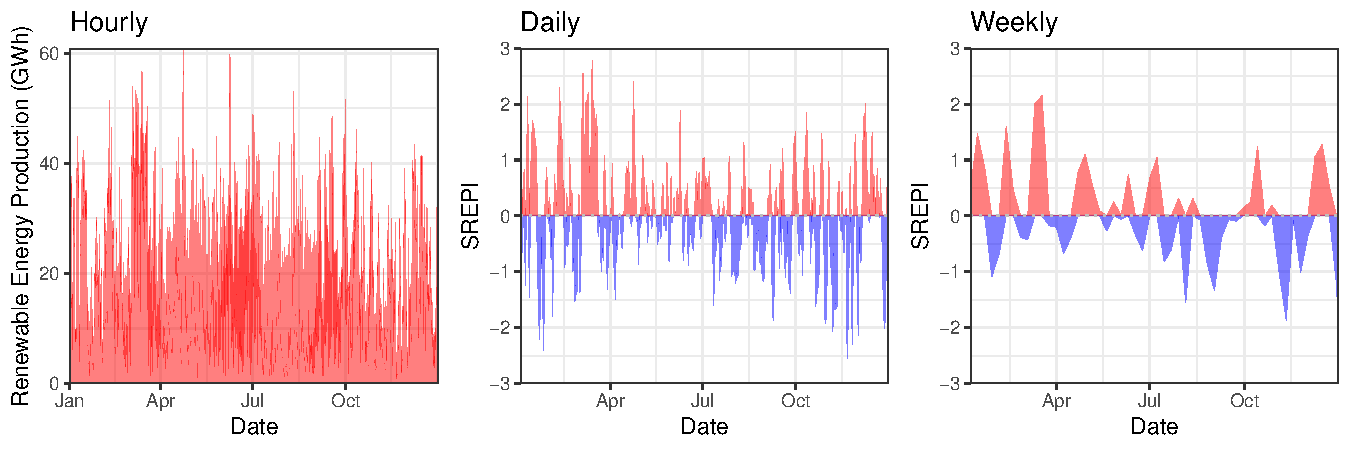
\includegraphics[width=\linewidth]{figure/plot_sei_ts-1} 

}


\end{knitrout}
\caption{Time series of 2019 SREPI values in Germany at hourly, daily, and weekly time scales.}
\label{fig:ts_si}
\end{figure}

By default, the \code{plot_sei()} function displays the time series of input values. However, by specifying \code{type = "hist"} (rather than the default \code{type = "ts"}), this function can additionally be used to plot a histogram of the input values. An example of this for the daily data production and corresponding SREPI values is presented in Figure \ref{fig:dist_raw}. As discussed in Section \ref{section:distribution}, such a plot can be used to validate the distributional assumptions made when calculating the indices. While the raw renewable energy production follows a heavily skewed distribution, the SREPI values resemble a sample from a standard normal distribution, suggesting the empirical distribution function is appropriate in this example. If probability or bounded indices were used, then the histogram of SREPI values should be flat, rather than normal. This is illustrated in Figure \ref{fig:dist_raw_unif}.


\begin{figure}
\begin{knitrout}
\definecolor{shadecolor}{rgb}{0.969, 0.969, 0.969}\color{fgcolor}\begin{kframe}
\begin{alltt}
\hlstd{plot_raw} \hlkwb{<-} \hlkwd{plot_sei}\hlstd{(de_supply_d,} \hlkwc{type} \hlstd{=} \hlstr{"hist"}\hlstd{,}
                     \hlkwc{lab} \hlstd{=} \hlstr{"Renewable Energy Production (GWh)"}\hlstd{)}
\hlstd{plot_ind} \hlkwb{<-} \hlkwd{plot_sei}\hlstd{(srepi_d,} \hlkwc{type} \hlstd{=} \hlstr{"hist"}\hlstd{,} \hlkwc{lab} \hlstd{=} \hlstr{"SREPI"}\hlstd{)}
\hlkwd{grid.arrange}\hlstd{(plot_raw, plot_ind,} \hlkwc{nrow} \hlstd{=} \hlnum{1}\hlstd{)}
\end{alltt}
\end{kframe}

{\centering 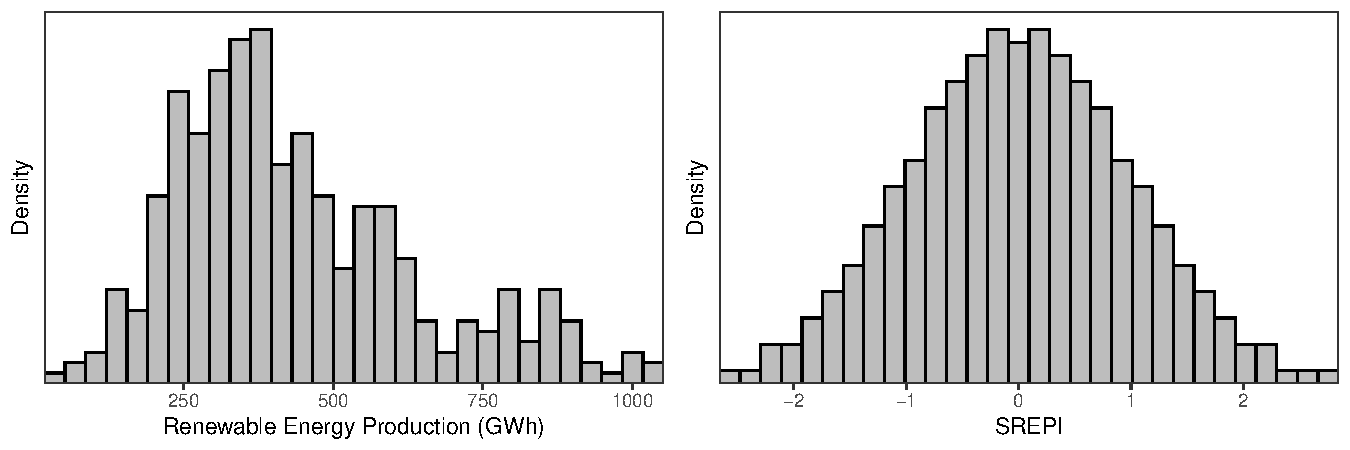
\includegraphics[width=\linewidth]{figure/plot_dist-1} 

}


\end{knitrout}
\caption{Histogram of 2019 daily renewable energy production and SREPI values in Germany.}
\label{fig:dist_raw}
\end{figure}

\begin{figure}
\begin{knitrout}
\definecolor{shadecolor}{rgb}{0.969, 0.969, 0.969}\color{fgcolor}\begin{kframe}
\begin{alltt}
\hlstd{srepi_d_prob} \hlkwb{<-} \hlkwd{std_index}\hlstd{(de_supply_d,} \hlkwc{index_type} \hlstd{=} \hlstr{"probability"}\hlstd{)}
\end{alltt}


{\ttfamily\noindent\bfseries\color{errorcolor}{\#\# Error in check\_inputs(inputs): index\_type must be one of 'normal', 'prob01', or 'prob11'}}\begin{alltt}
\hlstd{plot_prob} \hlkwb{<-} \hlkwd{plot_sei}\hlstd{(srepi_d_prob,} \hlkwc{type} \hlstd{=} \hlstr{"hist"}\hlstd{,} \hlkwc{lab} \hlstd{=} \hlstr{"SREPI"}\hlstd{,}
                      \hlkwc{ylims} \hlstd{=} \hlkwd{c}\hlstd{(}\hlnum{0}\hlstd{,} \hlnum{2}\hlstd{),} \hlkwc{title} \hlstd{=} \hlstr{"Probability"}\hlstd{)}
\end{alltt}


{\ttfamily\noindent\bfseries\color{errorcolor}{\#\# Error in eval(expr, envir, enclos): object 'srepi\_d\_prob' not found}}\begin{alltt}
\hlstd{srepi_d_bnd} \hlkwb{<-} \hlkwd{std_index}\hlstd{(de_supply_d,} \hlkwc{index_type} \hlstd{=} \hlstr{"bounded"}\hlstd{)}
\end{alltt}


{\ttfamily\noindent\bfseries\color{errorcolor}{\#\# Error in check\_inputs(inputs): index\_type must be one of 'normal', 'prob01', or 'prob11'}}\begin{alltt}
\hlstd{plot_bnd} \hlkwb{<-} \hlkwd{plot_sei}\hlstd{(srepi_d_bnd,} \hlkwc{type} \hlstd{=} \hlstr{"hist"}\hlstd{,} \hlkwc{lab} \hlstd{=} \hlstr{"SREPI"}\hlstd{,}
                     \hlkwc{ylims} \hlstd{=} \hlkwd{c}\hlstd{(}\hlnum{0}\hlstd{,} \hlnum{1}\hlstd{),} \hlkwc{title} \hlstd{=} \hlstr{"Bounded"}\hlstd{)}
\end{alltt}


{\ttfamily\noindent\bfseries\color{errorcolor}{\#\# Error in eval(expr, envir, enclos): object 'srepi\_d\_bnd' not found}}\begin{alltt}
\hlkwd{grid.arrange}\hlstd{(plot_prob, plot_bnd,} \hlkwc{nrow} \hlstd{=} \hlnum{1}\hlstd{)}
\end{alltt}


{\ttfamily\noindent\bfseries\color{errorcolor}{\#\# Error in eval(expr, envir, enclos): object 'plot\_prob' not found}}\end{kframe}
\end{knitrout}
\caption{Histogram of 2019 daily renewable energy production and SREPI values in Germany, where the indices are probability and bounded indices.}
\label{fig:dist_raw_unif}
\end{figure}

Finally, the \pkg{SEI} package additionally allows shortages or drought characteristics of the time series to be assessed. In this case, an energy supply drought could occur if the renewable energy production is low compared to previously observed values \citep{AllenOtero2023}. This corresponds to a low SREPI. As in Table \ref{tab:drought_def}, we define three categories of droughts, each defined using increasing thresholds of the SREPI. The function \code{get_drought()} can then be used to obtain a time series of drought occurrences, intensities, durations, and magnitudes.

\begin{knitrout}
\definecolor{shadecolor}{rgb}{0.969, 0.969, 0.969}\color{fgcolor}\begin{kframe}
\begin{alltt}
\hlstd{thresholds} \hlkwb{<-} \hlopt{-}\hlkwd{qnorm}\hlstd{(}\hlkwd{c}\hlstd{(}\hlnum{0.9}\hlstd{,} \hlnum{0.95}\hlstd{,} \hlnum{0.975}\hlstd{))} \hlcom{# -1.28, -1.64, -1.96}
\hlstd{drought_df} \hlkwb{<-} \hlkwd{get_drought}\hlstd{(srepi_d, thresholds,} \hlkwc{exceed} \hlstd{= F)}
\end{alltt}
\end{kframe}
\end{knitrout}

From the dataframe \code{drought_df}, it is straightforward to analyse the properties of these drought events. For example, we can list the frequency that a moderate, severe, or extreme drought event occurs,

\begin{knitrout}
\definecolor{shadecolor}{rgb}{0.969, 0.969, 0.969}\color{fgcolor}\begin{kframe}
\begin{alltt}
\hlstd{num_ev} \hlkwb{<-} \hlkwd{table}\hlstd{(drought_df}\hlopt{$}\hlstd{ins)}
\hlkwd{names}\hlstd{(num_ev)} \hlkwb{<-} \hlkwd{c}\hlstd{(}\hlstr{"None"}\hlstd{,} \hlstr{"Moderate"}\hlstd{,} \hlstr{"Severe"}\hlstd{,} \hlstr{"Extreme"}\hlstd{)}
\hlkwd{print}\hlstd{(num_ev)}
\end{alltt}
\begin{verbatim}
##     None Moderate   Severe  Extreme 
##      330       18        9        8
\end{verbatim}
\end{kframe}
\end{knitrout}

we could display the relative frequency of drought durations,
\begin{knitrout}
\definecolor{shadecolor}{rgb}{0.969, 0.969, 0.969}\color{fgcolor}\begin{kframe}
\begin{alltt}
\hlkwd{table}\hlstd{(drought_df}\hlopt{$}\hlstd{dur[drought_df}\hlopt{$}\hlstd{dur} \hlopt{>} \hlnum{0}\hlstd{])}
\end{alltt}
\begin{verbatim}
## 
##  1  2  3 
## 11  3  6
\end{verbatim}
\end{kframe}
\end{knitrout}

or we could calculate the average drought magnitude,
\begin{knitrout}
\definecolor{shadecolor}{rgb}{0.969, 0.969, 0.969}\color{fgcolor}\begin{kframe}
\begin{alltt}
\hlkwd{mean}\hlstd{(drought_df}\hlopt{$}\hlstd{mag[drought_df}\hlopt{$}\hlstd{mag} \hlopt{!=} \hlnum{0}\hlstd{])}
\end{alltt}
\begin{verbatim}
## [1] 2.985504
\end{verbatim}
\end{kframe}
\end{knitrout}

These are just simple examples of analyses that could be performed using the output of \code{get_drought()}. For a more thorough analysis, readers are referred to \cite{AllenOtero2023}.

\subsection{Wind speed}

Consider now a second application of standardised indices to weather and climate variables. While standardised indices are most commonly used to construct the SPI and SPEI, they can also be applied to other climate variables (see Section \ref{section:intro} for examples). In this section, we use the framework discussed herein to define standardised wind speed indices. Monitoring wind speed is crucial in many applications, including aviation safety, renewable energy planning, and the design and insurance of infrastructure.

Hourly estimates of near-surface (10m) wind speed are publicly available for several European countries between 1979 and 2019 \citep{HersbachEtAl2023}. As in \cite{OteroEtAl2022b}, we aggregate these wind speeds to get daily nationwide averages. Consistent with the previous application to renewable energy production, the analysis is restricted to Germany, and this subset of data is available from \pkg{SEI}. For clarity of visualisation, the following analysis is limited to the three year period between 2017 and 2019.

\begin{knitrout}
\definecolor{shadecolor}{rgb}{0.969, 0.969, 0.969}\color{fgcolor}\begin{kframe}
\begin{alltt}
\hlkwd{data}\hlstd{(}\hlstr{"data_wind_de"}\hlstd{,} \hlkwc{package} \hlstd{=} \hlstr{"SEI"}\hlstd{)}
\hlstd{data_wind_de} \hlkwb{<-} \hlkwd{subset}\hlstd{(data_wind_de,} \hlkwd{format}\hlstd{(date,} \hlstr{"%Y"}\hlstd{)} \hlopt{>=} \hlnum{2017}\hlstd{)}
\hlkwd{head}\hlstd{(data_wind_de)}
\end{alltt}
\begin{verbatim}
##             date   wsmean
## 13881 2017-01-01 3.461528
## 13882 2017-01-02 3.479744
## 13883 2017-01-03 5.391327
## 13884 2017-01-04 6.801471
## 13885 2017-01-05 3.822558
## 13886 2017-01-06 2.101849
\end{verbatim}
\end{kframe}
\end{knitrout}

As before, the data can be rescaled using \pkg{xts} functionality to obtain time series of the weekly and monthly average wind speed in Germany. We label the resulting daily, weekly, and monthly time series \code{de_wind_d}, \code{de_wind_w}, and \code{de_wind_m}, respectively, all of which are \pkg{xts} objects. These time series are displayed using \code{plot_sei()} in Figure \ref{fig:ts_ws_raw}.



\begin{figure}
\begin{knitrout}
\definecolor{shadecolor}{rgb}{0.969, 0.969, 0.969}\color{fgcolor}\begin{kframe}
\begin{alltt}
\hlstd{lab} \hlkwb{<-} \hlstr{"Wind speed (m/s)"}
\hlstd{ylims} \hlkwb{<-} \hlkwd{c}\hlstd{(}\hlnum{0}\hlstd{,} \hlnum{8}\hlstd{)}
\hlstd{plot_ws_d} \hlkwb{<-} \hlkwd{plot_sei}\hlstd{(de_wind_d,} \hlkwc{lab} \hlstd{= lab,} \hlkwc{ylims} \hlstd{= ylims,} \hlkwc{title} \hlstd{=} \hlstr{"Daily"}\hlstd{)}
\hlstd{plot_ws_w} \hlkwb{<-} \hlkwd{plot_sei}\hlstd{(de_wind_w,} \hlkwc{lab} \hlstd{= lab,} \hlkwc{ylims} \hlstd{= ylims,} \hlkwc{title} \hlstd{=} \hlstr{"Weekly"}\hlstd{)}
\hlstd{plot_ws_m} \hlkwb{<-} \hlkwd{plot_sei}\hlstd{(de_wind_m,} \hlkwc{lab} \hlstd{= lab,} \hlkwc{ylims} \hlstd{= ylims,} \hlkwc{title} \hlstd{=} \hlstr{"Monthly"}\hlstd{)}
\hlkwd{grid.arrange}\hlstd{(plot_ws_d, plot_ws_w, plot_ws_m,} \hlkwc{nrow} \hlstd{=} \hlnum{1}\hlstd{)}
\end{alltt}
\end{kframe}

{\centering 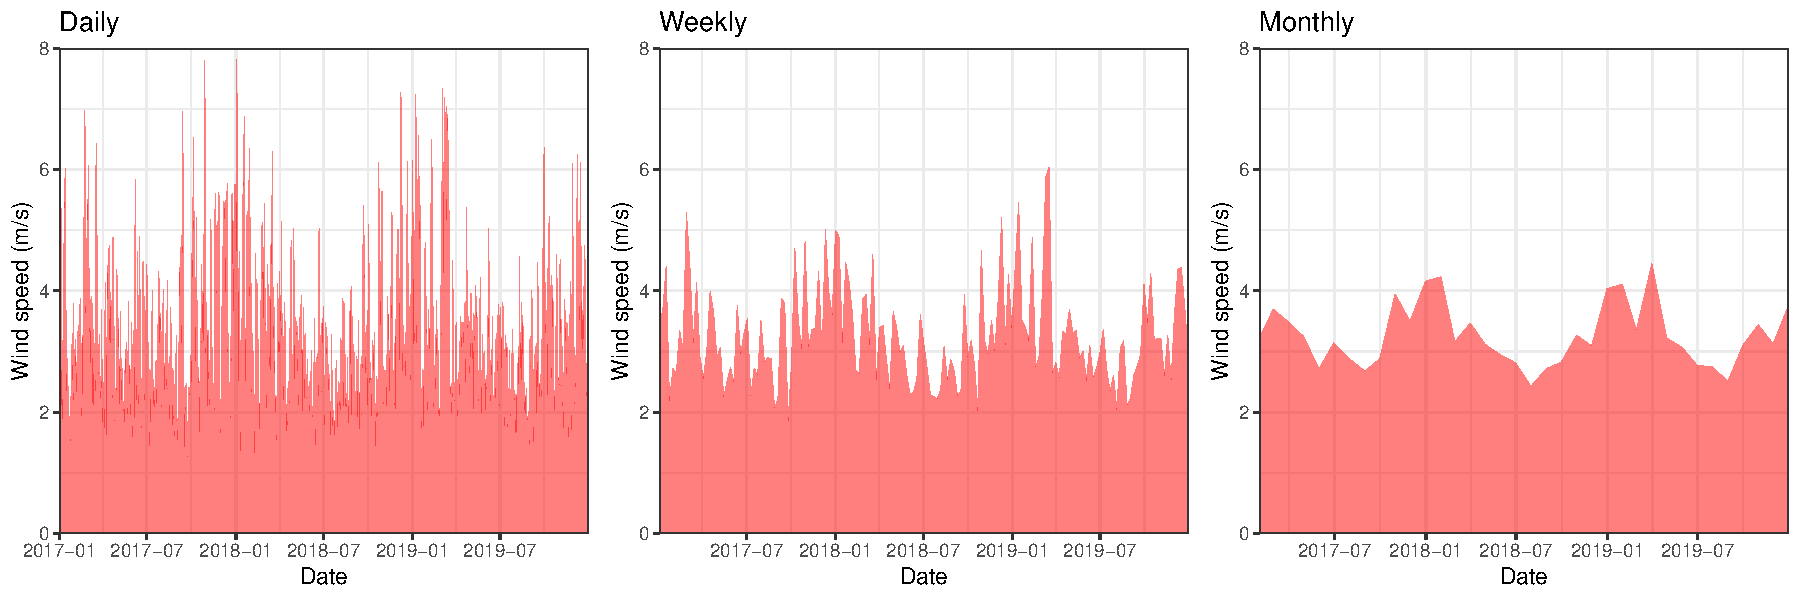
\includegraphics[width=\linewidth]{figure/plot_raw_ts_wind-1} 

}


\end{knitrout}
\caption{Daily, weekly and monthly time series of average wind speed in Germany between 2017 and 2019.}
\label{fig:ts_ws_raw}
\end{figure}

The raw data can be transformed to a time series of standardised indices using \code{std_index()}. As discussed, constructing standardised indices requires estimating the distribution of the variable of interest. While we argue that the empirical distribution provides a flexible means to achieve this, we demonstrate in this application how the \pkg{SEI} package allows parametric distributions to be used for this purpose.

Various distributions can be fit to the daily wind speeds using the \code{fit_dist()} function. Consider, for example, a gamma distribution, log-normal distribution, and Weibull distribution.

\begin{knitrout}
\definecolor{shadecolor}{rgb}{0.969, 0.969, 0.969}\color{fgcolor}\begin{kframe}
\begin{alltt}
\hlstd{out_gamma} \hlkwb{<-} \hlkwd{fit_dist}\hlstd{(data_wind_de}\hlopt{$}\hlstd{wsmean,} \hlkwc{dist} \hlstd{=} \hlstr{"gamma"}\hlstd{)}
\hlstd{out_lnorm} \hlkwb{<-} \hlkwd{fit_dist}\hlstd{(data_wind_de}\hlopt{$}\hlstd{wsmean,} \hlkwc{dist} \hlstd{=} \hlstr{"lnorm"}\hlstd{)}
\hlstd{out_weibull} \hlkwb{<-} \hlkwd{fit_dist}\hlstd{(data_wind_de}\hlopt{$}\hlstd{wsmean,} \hlkwc{dist} \hlstd{=} \hlstr{"weibull"}\hlstd{)}
\end{alltt}
\end{kframe}
\end{knitrout}

The three distributions can be compared with respect to their AIC, which is output from \code{fit_dist()}.

\begin{knitrout}
\definecolor{shadecolor}{rgb}{0.969, 0.969, 0.969}\color{fgcolor}\begin{kframe}
\begin{alltt}
\hlstd{aic_vec} \hlkwb{<-} \hlkwd{c}\hlstd{(out_gamma}\hlopt{$}\hlstd{fit_props[}\hlstr{'aic'}\hlstd{],}
             \hlstd{out_lnorm}\hlopt{$}\hlstd{fit_props[}\hlstr{'aic'}\hlstd{],}
             \hlstd{out_weibull}\hlopt{$}\hlstd{fit_props[}\hlstr{'aic'}\hlstd{])}
\hlkwd{names}\hlstd{(aic_vec)} \hlkwb{<-} \hlkwd{c}\hlstd{(}\hlstr{"Gamma"}\hlstd{,} \hlstr{"Log-normal"}\hlstd{,} \hlstr{"Weibull"}\hlstd{)}
\end{alltt}


{\ttfamily\noindent\bfseries\color{errorcolor}{\#\# Error in names(aic\_vec) <- c("{}Gamma"{}, "{}Log-normal"{}, "{}Weibull"{}): attempt to set an attribute on NULL}}\begin{alltt}
\hlkwd{print}\hlstd{(aic_vec)}
\end{alltt}
\begin{verbatim}
## NULL
\end{verbatim}
\end{kframe}
\end{knitrout}

The AIC provides a measure of distributional fit whilst also accounting for model complexity, with a smaller value indicating a better bit. The AIC values above suggest that the log-normal distribution provides the best fit to the data, while the Weibull distribution provides the worst fit.

This can be verified by looking at p-values corresponding to the Kolmogorov-Smirnov test.

\begin{knitrout}
\definecolor{shadecolor}{rgb}{0.969, 0.969, 0.969}\color{fgcolor}\begin{kframe}
\begin{alltt}
\hlstd{ksp_vec} \hlkwb{<-} \hlkwd{c}\hlstd{(out_gamma}\hlopt{$}\hlstd{fit_props[}\hlstr{'ks_pval'}\hlstd{],}
             \hlstd{out_lnorm}\hlopt{$}\hlstd{fit_props[}\hlstr{'ks_pval'}\hlstd{],}
             \hlstd{out_weibull}\hlopt{$}\hlstd{fit_props[}\hlstr{'ks_pval'}\hlstd{])}
\hlkwd{names}\hlstd{(ksp_vec)} \hlkwb{<-} \hlkwd{c}\hlstd{(}\hlstr{"Gamma"}\hlstd{,} \hlstr{"Log-normal"}\hlstd{,} \hlstr{"Weibull"}\hlstd{)}
\end{alltt}


{\ttfamily\noindent\bfseries\color{errorcolor}{\#\# Error in names(ksp\_vec) <- c("{}Gamma"{}, "{}Log-normal"{}, "{}Weibull"{}): attempt to set an attribute on NULL}}\begin{alltt}
\hlkwd{print}\hlstd{(}\hlkwd{round}\hlstd{(ksp_vec,} \hlnum{4}\hlstd{))}
\end{alltt}


{\ttfamily\noindent\bfseries\color{errorcolor}{\#\# Error in round(ksp\_vec, 4): non-numeric argument to mathematical function}}\end{kframe}
\end{knitrout}

The null hypothesis is that the sample of data has been drawn from the parametric distribution. The Kolmogorov-Smirnov test is rejected at the 0.5\% level for both the gamma and Weibull distributions, providing evidence to suggest that these distributions do not accurately describe the data. On the other hand, there is insufficient evidence to reject the null hypothesis that the wind speed data was drawn from a log-normal distribution.

The fit of the three distributions to the data is presented in Figure \ref{fig:dist_ws}. The \code{plot_sei()} function can be used to plot histograms of the daily wind speeds. Since \code{plot_sei()} returns a \pkg{ggplot2} object, the estimated density functions can be added to the histograms. For example, for the gamma distribution

\begin{knitrout}
\definecolor{shadecolor}{rgb}{0.969, 0.969, 0.969}\color{fgcolor}\begin{kframe}
\begin{alltt}
\hlstd{x} \hlkwb{<-} \hlkwd{seq}\hlstd{(}\hlnum{0}\hlstd{,} \hlnum{9}\hlstd{,} \hlkwc{length.out} \hlstd{=} \hlkwd{length}\hlstd{(de_wind_d))}
\hlstd{xlab} \hlkwb{<-} \hlstr{"Wind speed (m/s)"}
\hlstd{pars_gam} \hlkwb{<-} \hlstd{out_gamma}\hlopt{$}\hlstd{params}

\hlstd{plt_gam} \hlkwb{<-} \hlkwd{plot_sei}\hlstd{(de_wind_d,} \hlkwc{type} \hlstd{=} \hlstr{"hist"}\hlstd{,} \hlkwc{lab} \hlstd{= xlab,} \hlkwc{title} \hlstd{=} \hlstr{"Gamma"}\hlstd{)} \hlopt{+}
  \hlkwd{geom_line}\hlstd{(}\hlkwd{aes}\hlstd{(}\hlkwc{x} \hlstd{= x,} \hlkwc{y} \hlstd{=} \hlkwd{dgamma}\hlstd{(x, pars_gam[}\hlnum{1}\hlstd{], pars_gam[}\hlnum{2}\hlstd{])),} \hlkwc{col} \hlstd{=} \hlstr{"blue"}\hlstd{)}
\end{alltt}
\end{kframe}
\end{knitrout}


\begin{figure}
\begin{knitrout}
\definecolor{shadecolor}{rgb}{0.969, 0.969, 0.969}\color{fgcolor}

{\centering 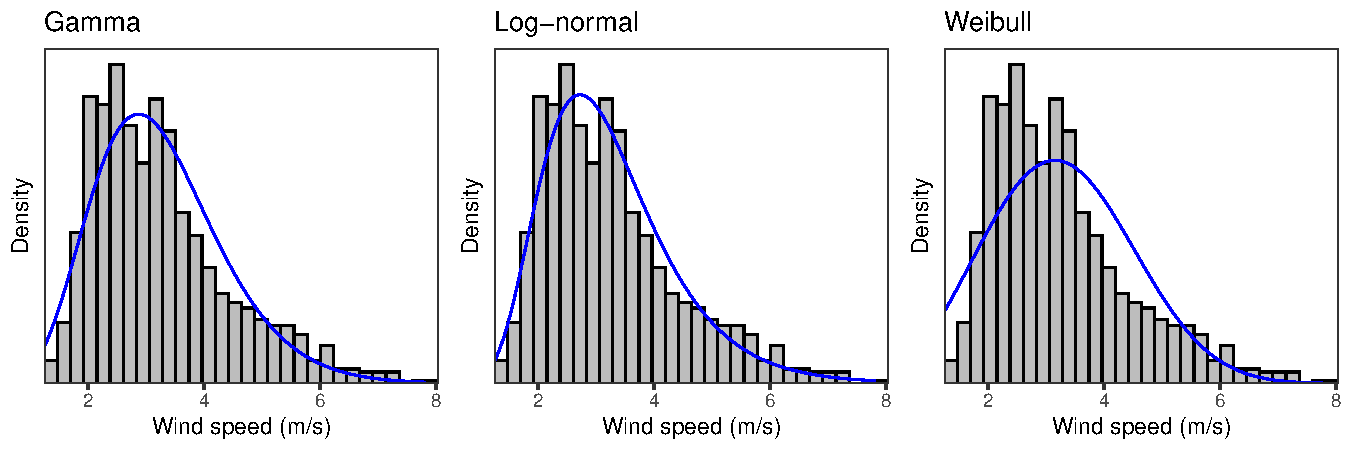
\includegraphics[width=\linewidth]{figure/ws_plot_dist-1} 

}


\end{knitrout}
\caption{Distribution of daily wind speeds in Germany between 2017 and 2019, along with estimated gamma, log-normal, and Weibull densities.}
\label{fig:dist_ws}
\end{figure}

Finally, the adequacy of the distributions can also be visualised by plotting a histogram of the standardised indices obtained using the three distributions. The standardised indices can be calculated using the \code{std_index()} function, with the \code{dist} argument corresponding to the distribution of interest.

\begin{knitrout}
\definecolor{shadecolor}{rgb}{0.969, 0.969, 0.969}\color{fgcolor}\begin{kframe}
\begin{alltt}
\hlstd{sei_ws_gam} \hlkwb{<-} \hlkwd{std_index}\hlstd{(de_wind_d,} \hlkwc{dist} \hlstd{=} \hlstr{"gamma"}\hlstd{)}
\hlstd{sei_ws_lnorm} \hlkwb{<-} \hlkwd{std_index}\hlstd{(de_wind_d,} \hlkwc{dist} \hlstd{=} \hlstr{"lnorm"}\hlstd{)}
\hlstd{sei_ws_weib} \hlkwb{<-} \hlkwd{std_index}\hlstd{(de_wind_d,} \hlkwc{dist} \hlstd{=} \hlstr{"weibull"}\hlstd{)}
\end{alltt}
\end{kframe}
\end{knitrout}

Histograms of the standardised indices, constructed using \code{plot_sei()}, are displayed in Figure \ref{fig:dist_ws_ind}. Similarly to before, a standard normal distribution is superimposed onto the histograms.

\begin{figure}
\begin{knitrout}
\definecolor{shadecolor}{rgb}{0.969, 0.969, 0.969}\color{fgcolor}

{\centering 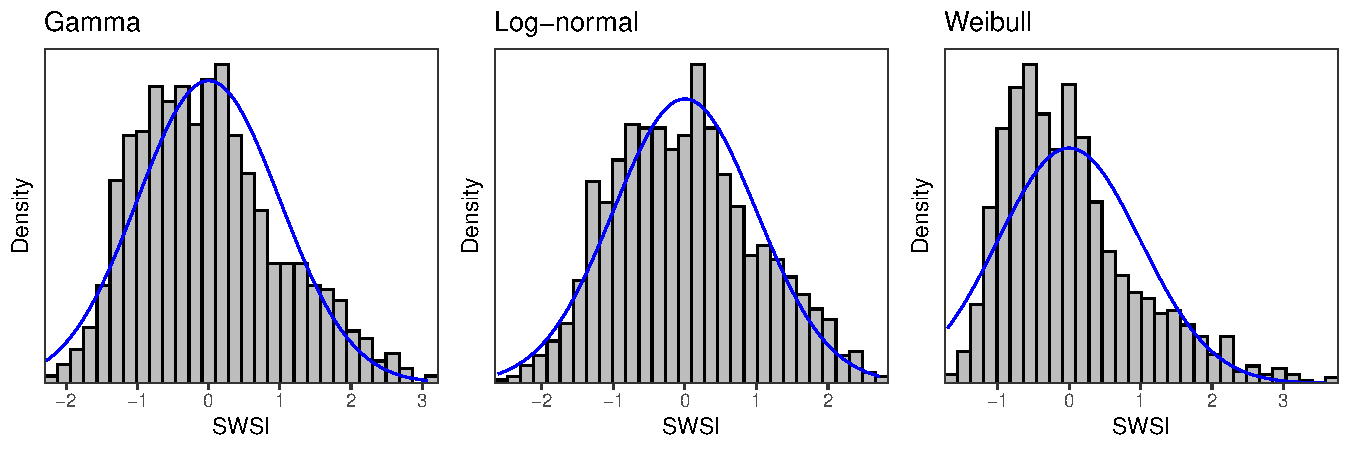
\includegraphics[width=\linewidth]{figure/ws_ind_plot_dist-1} 

}


\end{knitrout}
\caption{Distribution of standardised wind speed indices (SWSI) constructed using the gamma, log-normal, and Weibull distributions. The standard normal density is displayed in blue.}
\label{fig:dist_ws_ind}
\end{figure}

As expected, no parametric distribution fits the data perfectly. The standardised wind speed indices constructed using a log-normal distribution appear closer to a standard normal distribution, reinforcing the previous conclusions that this distribution provides a more accurate fit to the daily wind speed data.

Having constructed these wind speed indices, it would be straightforward to conduct an analysis of wind droughts (or extreme wind speeds) using the \code{get_drought()} function in \pkg{SEI}, akin to how renewable energy production droughts were studied in the previous application. This is omitted here for concision, but could be analysed in more detail in the future.


\section{Summary}\label{section:conclusion}

This vignette documents the \pkg{SEI} package in \proglang{R}, which provides comprehensive functionality to calculate time series of standardised indices. Standardised indices are projections of variables onto an interpretable and probabilistically meaningful scale, and they have become popular tools when monitoring variables of interest over time, particularly in the context of drought analysis. While there is no unique way to define standardised indices, several widely-adopted indices are constructed using the same, simple procedure. We outline this general framework for constructing standardised indices, and reiterate that this approach can be applied to any variable of interest, not just those previously considered in the literature.

The \pkg{SEI} package converts a time series of observations to a time series of standardised indices. The package allows the time series to be aggregated and rescaled to different time scales, provides plot capabilities to visualise the resulting indices, and offers a range of distributions with which to calculate the indices, including flexible non- and semi-parametric methods. The package additionally allows users to define and analyse shortages, or droughts, of the variable under consideration. Two examples are presented in Section \ref{section:application} whereby the package is employed to calculate standardised indices to monitor shortages in renewable energy production, and to calculate standardised wind speed indices.

The package has been designed to facilitate applications of standardised indices in practice. While standardised indices have received considerable attention within the field of climate science, such indices would also be relevant in several other domains. The \pkg{SEI} package is applicable in broad generality, though the package could also be extended so that it is suitable for more elaborate analyses. For example, several extensions of standardised indices have been proposed in the literature, and these could be integrated into the package: the package currently only considers indices corresponding to univariate variables, though multivariate extensions have also been studied in the literature \citep[e.g.][]{ErhardtCzado2018,HaoEtAl2019}; non-stationary standardised indices have also been proposed that allow the indices to depend on covariates \citep{RussoEtAl2013,LiEtAl2015}; functionality could also be added to automatically implement methods that remove seasonality and temporal dependence in the data \citep{ErhardtCzado2018}. %The data could be divided into several time series corresponding to each month or season, and the standardisation performed separately, before recombining the resulting time series; currently, this must be performed manually by the user.


Moreover, while the package extends existing packages by providing flexible density estimation methods, alternative such methods could also be made available, particularly methods that are appropriate when estimating the distribution of bounded variables. Functionality could also be added to handle spatial data, and, finally, the functionality of the package could be transferred to software packages in other programming languages, facilitating the implementation of standardised indices in monitoring systems that have not been designed in \proglang{R}.

\section*{Acknowledgements}

This package was created under funding by the Oeschger Centre for Climate Change Research and the Swiss Federal Office of Meteorology and Climatology (MeteoSwiss).

%% Bibliography
\bibliography{bibliography}

\end{document}

